\documentclass[11pt,a4paper]{article}
\usepackage[T1]{fontenc}
\usepackage[utf8]{inputenc}
\usepackage{lmodern,amsmath,amssymb,amsthm,microtype}
\usepackage[margin=27mm]{geometry}
\usepackage[dvipsnames]{xcolor}
\usepackage[colorlinks=true,urlcolor=MidnightBlue,citecolor=MidnightBlue,linkcolor=MidnightBlue]{hyperref}
\usepackage{tikz,booktabs}
\usetikzlibrary{arrows.meta,automata,positioning}
\newtheorem{theorem}{Theorem}
\newtheorem{lemma}[theorem]{Lemma}
\newcommand{\rk}{\operatorname{rk}}
\newcommand{\gen}[1]{\langle #1\rangle}
\title{A rank-drop counterexample\protect\\ to Kourovka Problem 20.8}
\author{AI-generated mathematical note}
\date{Version 1 --- 6 November 2026}
\begin{document}
\maketitle
\begin{center}\small\textbf{Candidate solution --- review pending.}\end{center}
\begin{abstract}
We give an explicit negative answer to the homomorphism-uniqueness question in Kourovka Problem 20.8. There are free groups $K<H<F$ of ranks $4,3,2$, respectively, such that every proper subgroup of $H$ containing $K$ has rank at least four, while a homomorphism $H\to F$ fixes $K$ pointwise and differs from inclusion. The example specializes Lei and Zhang's existing equalizer construction. We verify the additional intermediate-subgroup condition directly with a three-vertex Schreier-graph argument. Priority for this application is not established; no human acceptance or formal verification is claimed.
\end{abstract}

\section{The question and the example}
Problem 20.8, proposed by G.~M.~Bergman, asks whether the following hypotheses imply that inclusion is the only homomorphism $H\to F$ fixing $K$ pointwise: $K<H<F$ are free groups of finite rank, $\rk(H)<\rk(K)$, and every proper subgroup $L<H$ containing $K$ satisfies $\rk(L)\geq\rk(K)$ \cite{Kourovka}. Here rank means free-basis rank. The intermediate subgroup $L$ need not be finitely generated.

Let $F=F(a,b)$ be the free group on $a,b$, and define
\[
u=(a^{-1}b)^2,\qquad v=(a^{-2}b^2)^2,
\]
\[
H=\gen{a,u,v},\qquad K=\gen{u,v,aua^{-1},a^2va^{-2}}.
\]
\begin{theorem}\label{thm:main}
The inclusions $K<H<F$ are strict, and the three groups have ranks $4,3,2$, respectively. Every $K\leq L<H$ has rank at least four. The assignment
\[
\phi(a)=b,\qquad \phi(u)=u,\qquad \phi(v)=v
\]
defines a homomorphism $\phi:H\to F$ fixing $K$ pointwise and differing from inclusion. Consequently, the answer to Problem 20.8 is negative.
\end{theorem}

The words and subgroup pattern come from the rank-three instance of Lei and Zhang's construction \cite[Proposition 3.3 and Construction 4.1]{LZ}. We credit that construction to them. The additional assertion to verify here is the rank bound for \emph{every proper intermediate subgroup}; a large equalizer alone would not establish this assertion for a specified subgroup. The proof below verifies the required data without assuming their full equalizer-rank theorem or the project's proposed solution of Problem 20.11.

\section{The two rank calculations}
We use graphs whose edges are labelled by elements of a free basis and their inverses. Reversing an edge reverses its label. A graph is \emph{folded} if at each vertex there is at most one outgoing edge with any prescribed signed label. A reduced path in a folded graph has a freely reduced label, so labelling induces an injection of its fundamental group into the free group. A finite connected graph with $E$ topological edges and $V$ vertices has free rank $E-V+1$. Each topological edge is counted once, not twice for its two orientations.

\begin{lemma}\label{lem:H}
The ordered triple $(a,u,v)$ is a free basis of $H$, and $\rk(H)=3$.
\end{lemma}
\begin{proof}
Put $d_1=au=ba^{-1}b$ and $d_2=a^2v=b^2a^{-2}b^2$. Consider the following graph, based at $o$. The displayed arrows specify one orientation of each edge; inverse orientations are understood.
\begin{center}
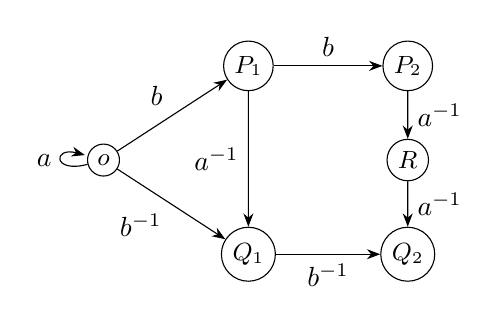
\begin{tikzpicture}[>=Stealth,vertex/.style={circle,draw,fill=white,inner sep=2pt,font=\small},every edge/.style={draw,->},scale=0.92]
\node[vertex] (o) at (0,0) {$o$};
\node[vertex] (p1) at (2,1.3) {$P_1$};
\node[vertex] (p2) at (4.2,1.3) {$P_2$};
\node[vertex] (q1) at (2,-1.3) {$Q_1$};
\node[vertex] (q2) at (4.2,-1.3) {$Q_2$};
\node[vertex] (r) at (4.2,0) {$R$};
\path (o) edge[loop left] node[left] {$a$} (o)
 (o) edge node[above left] {$b$} (p1)
 (p1) edge node[above] {$b$} (p2)
 (o) edge node[below left] {$b^{-1}$} (q1)
 (q1) edge node[below] {$b^{-1}$} (q2)
 (p1) edge node[left] {$a^{-1}$} (q1)
 (p2) edge node[right] {$a^{-1}$} (r)
 (r) edge node[right] {$a^{-1}$} (q2);
\end{tikzpicture}
\end{center}
At every vertex the outgoing signed labels are distinct, so the graph is folded. It has six vertices and eight topological edges. The four $b$-edges and the edge $P_2\to R$ form a spanning tree. The three remaining edges yield based loops labelled $a,d_1,d_2$. Thus these elements freely generate the represented subgroup, of rank $8-6+1=3$.

This subgroup is $H$, because $d_1=au$, $d_2=a^2v$, and conversely $u=a^{-1}d_1$, $v=a^{-2}d_2$. Replacing $d_1,d_2$ by $a^{-1}d_1,a^{-2}d_2$ is an invertible Nielsen change of basis fixing $a$. Hence $(a,u,v)$ is a free basis of $H$.
\end{proof}

\begin{lemma}\label{lem:K}
The group $K$ has rank four.
\end{lemma}
\begin{proof}
Use the basis $(a,u,v)$ of $H$. The following connected folded graph $\Gamma$ is based at vertex $0$:
\begin{center}
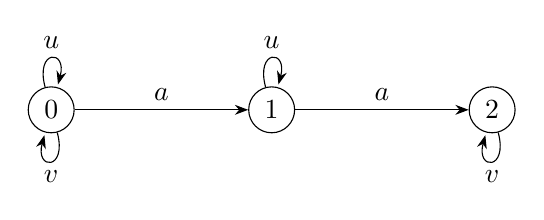
\begin{tikzpicture}[>=Stealth,vertex/.style={circle,draw,fill=white,inner sep=3pt},every edge/.style={draw,->}]
\node[vertex] (v0) at (0,0) {$0$};
\node[vertex] (v1) at (2.8,0) {$1$};
\node[vertex] (v2) at (5.6,0) {$2$};
\path (v0) edge node[above] {$a$} (v1)
 (v1) edge node[above] {$a$} (v2)
 (v0) edge[loop above] node[above] {$u$} (v0)
 (v1) edge[loop above] node[above] {$u$} (v1)
 (v0) edge[loop below] node[below] {$v$} (v0)
 (v2) edge[loop below] node[below] {$v$} (v2);
\end{tikzpicture}
\end{center}
The two $a$-edges form a spanning tree, and the four complementary loops yield exactly $u,v,aua^{-1},a^2va^{-2}$. Thus $\Gamma$ represents $K$ and has rank $6-3+1=4$.
\end{proof}

\section{The condition on every intermediate subgroup}
\begin{lemma}\label{lem:intermediate}
For every subgroup $L$ with $K\leq L<H$, one has $\rk(L)\geq4$.
\end{lemma}
\begin{proof}
Take the right-coset Schreier graph of $L$ in $H$ with respect to $(a,u,v)$. Its vertices are $Lw$, with an $x$-edge $Lw\to Lwx$ for each basis element $x$. Its fundamental group, based at $L$, identifies with $L$.

Set $z_0=L$, $z_1=La$, and $z_2=La^2$. The six edges of $\Gamma$ occur on these vertices. In particular the $u$-loop at $z_1$ exists because $aua^{-1}\in L$, and the $v$-loop at $z_2$ exists because $a^2va^{-2}\in L$.

If $z_0=z_1$, then $a\in L$. Together with $u,v\in K\leq L$, this gives $L=H$, a contradiction. If $z_1=z_2$, the right-coset equality implies $a(a^2)^{-1}=a^{-1}\in L$, giving the same contradiction. Thus consecutive vertices are distinct. There are precisely two remaining cases.

If all three vertices are distinct, the six displayed edges form an embedded connected subgraph of rank $6-3+1=4$. Their labels, endpoints, and orientations distinguish the topological edges in the Schreier graph.

If $z_0=z_2$, while $z_1$ is distinct, the two $v$-loops coincide. The remaining image has two $a$-edges in a two-edge cycle, one $u$-loop at each vertex, and one $v$-loop at $z_0$. In particular the two $a$-edges are distinct topological edges: each has positive label $a$, whereas reversing an edge changes its label to $a^{-1}$. There are five edges and two vertices, giving rank $5-2+1=4$.

In either case the Schreier graph contains an embedded subgraph with four independent cycles. Such cycles remain independent in the whole graph: graphs have no two-dimensional boundaries in homology. Hence the graph fundamental group $L$ has rank at least four. This argument applies equally when the Schreier graph or the rank of $L$ is infinite.
\end{proof}

The embedding of the displayed \emph{subgraph} is essential. We are not invoking rank monotonicity for arbitrary subgroup inclusions, which is false for free groups.

\section{The homomorphism and conclusion}
By Lemma~\ref{lem:H}, the values $\phi(a)=b$, $\phi(u)=u$, $\phi(v)=v$ define a homomorphism on $H$. For $i=1,2$ put $c_i=a^{-i}b^i$, so that $u=c_1^2$, $v=c_2^2$, and $b^i=a^ic_i$. Then
\[
b^ic_i^2b^{-i}
=a^ic_i c_i^2 c_i^{-1}a^{-i}
=a^ic_i^2a^{-i}.
\]
Thus $\phi$ fixes $aua^{-1}$ and $a^2va^{-2}$ as well as $u,v$. It therefore fixes $K$ pointwise. However, $\phi(a)=b\ne a$, so it differs from inclusion.

The ranks of $K,H,F$ are $4,3,2$, respectively. In particular the inclusions are strict and $\rk(H)<\rk(K)$. Lemma~\ref{lem:intermediate} verifies the remaining hypothesis of the original question. This proves Theorem~\ref{thm:main}.

\section{Evidence, attribution, and review status}
An accompanying Python script uses exact free reduction and finite Stallings folding. It checks the rank of $H$ in $F(a,b)$, the rank of $K$ relative to $(a,u,v)$, and the rank of $K$ directly in $F(a,b)$, obtaining $3,4,4$. It checks agreement of the two homomorphisms on all four generators of $K$, disagreement on $a$, and that $b\notin H$. All five partitions of the vertices of $\Gamma$ give the following folded graphs:
\begin{center}
\begin{tabular}{lrrr}
\toprule
Initial identification & Vertices & Edges & Rank\\
\midrule
None & 3 & 6 & 4\\
$0=1$ & 1 & 3 & 3\\
$0=2$ & 2 & 5 & 4\\
$1=2$ & 1 & 3 & 3\\
$0=1=2$ & 1 & 3 & 3\\
\bottomrule
\end{tabular}
\end{center}
Every rank-three quotient is the full three-petal rose representing $H$. These computations check finite proof data; the universal assertion about intermediate subgroups is proved in Lemma~\ref{lem:intermediate}, not by a finite search alone. The script uses only the Python standard library and was run with Python 3.12.14. The archived evidence includes its complete output.

The original words and graph pattern are due to Lei and Zhang. This note gives an explicit application to the exact hypotheses of Kourovka 20.8, with a direct verification of the extra intermediate-subgroup condition. The November 2026 entry is unmarked, but that does not establish worldwide openness or priority. This deduction may already be known to specialists.

This manuscript was generated by ChatGPT/Codex. A separate Codex reviewer audited the exact archived argument and found no mathematical gap; no repair was needed. Human mathematical review remains pending. The accompanying review record gives the audit's exact scope and includes the reproducibility script and its output. No Lean executable was available; no Lean formalization or machine-checked proof is supplied. Repository checks and model agreement are not human acceptance. No public conversation link was supplied, and no private transcript is included.

The candidate is archived as claim C1 at commit \texttt{b878477e0c53}. The accompanying review notes record the full run and commit identifiers, source hashes, and the precise version inspected.

\begin{thebibliography}{9}
\bibitem{Kourovka} E.~I.~Khukhro and V.~D.~Mazurov (eds.), \emph{The Kourovka Notebook: Unsolved Problems in Group Theory}, No.~21, November 2026 update, Problem 20.8, p.~157.\par\url{https://kourovkanotebookorg.wordpress.com/wp-content/uploads/2026/11/21tkt.pdf}
\bibitem{LZ} J.~Lei and T.~Zhang, \emph{Colored Stallings graphs and counterexamples to the Stallings equalizer conjecture}, arXiv:2604.24502v2 (9 May 2026), Proposition 3.3 and Construction 4.1.\par\url{https://arxiv.org/pdf/2604.24502v2}
\end{thebibliography}
\end{document}
